\documentclass{article}

\usepackage[spanish]{babel}
\usepackage[utf8]{inputenc}
\usepackage{fullpage}
\usepackage{graphicx}

\title{
    \LARGE{PyTiger2C} \\
    \Large{Documentación de la interfaz gráfica}
}

\author{
    Yasser González Fernández \\
    \small{yglez@uh.cu}
    \and
    Ariel Hernández Amador \\
    \small{gnuaha7@uh.cu}
}

\date{}

\begin{document}

\maketitle

\thispagestyle{empty}

\newpage

\setcounter{page}{1}

Este documento muestra, de manera general, los pasos a seguir para crear un
nuevo programa Tiger utilizando la interfaz gráfica de PyTiger2C. Además,
ilustra otras funcionalidades de la interfaz gráfica como la posibilidad de
mostrar el árbol de sintáxis abstracta correspondiente al programa y
el código C generado.

La interfaz gráfica puede iniciarse ejecutando el \emph{script} Python
\texttt{gpytiger2c.py} que se encuentra en el directorio \texttt{scripts}
de la distribución en código fuente de PyTiger2C.

Al ejecutar este \emph{script}, se mostrará la ventana principal de la interfaz
gráfica como se ilustra en la figura~\ref{fig:1-main-window}.

\begin{figure}[htb]
  \centering
  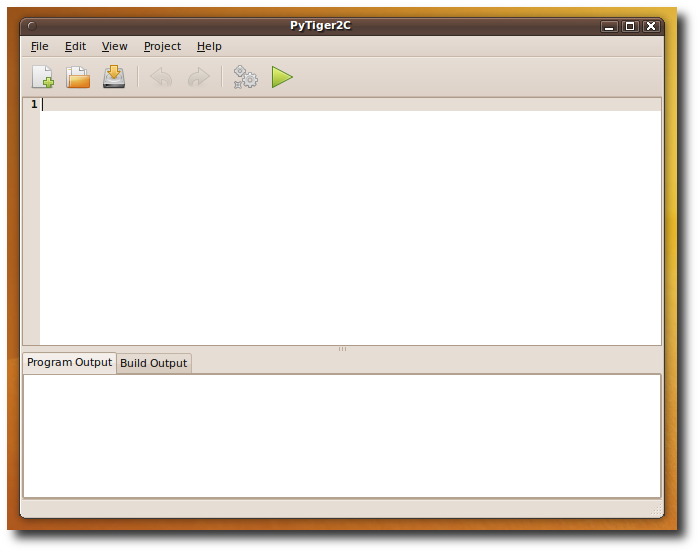
\includegraphics[width=5.5in]{gui/1-main-window}
  \caption{Ventana principal.}
  \label{fig:1-main-window}
\end{figure}

El elemento principal de esta ventana es el control \emph{GtkSorceViewer} que
permite introducir el código fuente del programa en el lenguaje Tiger. Este
control brinda las siguientes funcionalidades: resaltado de sintáxis a partir
de una descripción de la estructura del lenguaje mediante un archivo XML,
permite deshacer y rehacer los cambios hechos durante la edición, muestra el
número de cada línea del archivo y resalta la línea donde se encuentra el cursor
y los caracteres que deben una pareja como paréntesis, llaves y corchetes.

\newpage

Las funcionalidades disponibles durante la edición descritas anteriormente se
ilustran en la figura~\ref{fig:2-editing} con una implementación del conocido
programa \emph{Hello, World!} en el lenguaje Tiger.

\begin{figure}[htb]
  \centering
  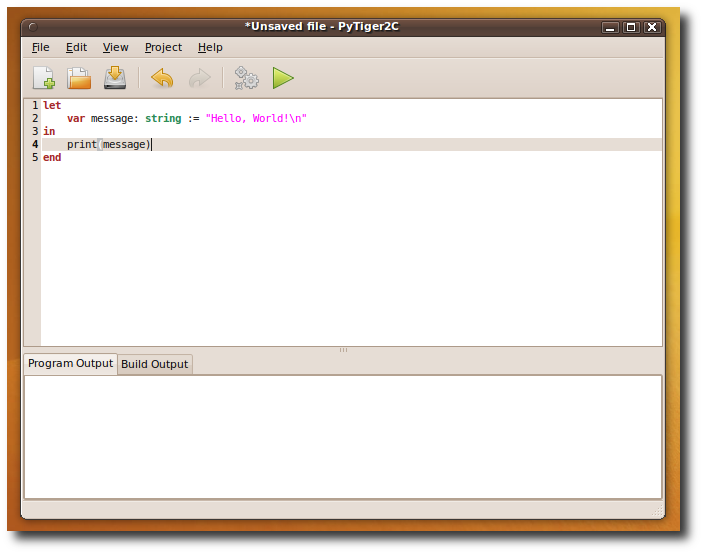
\includegraphics[width=5.5in]{gui/2-editing}
  \caption{Creación de un programa.}
  \label{fig:2-editing}
\end{figure}

\newpage

Luego de terminada la edición del nuevo programa Tiger y antes de efectuar
su compilación se debe guardar el programa en un nuevo archivo. Para hacer
esto se puede utilizar el elemento \emph{Save As...} del menú \emph{File}
como se ilustra en la figura~\ref{fig:3-saving-as}.

\begin{figure}[htb]
  \centering
  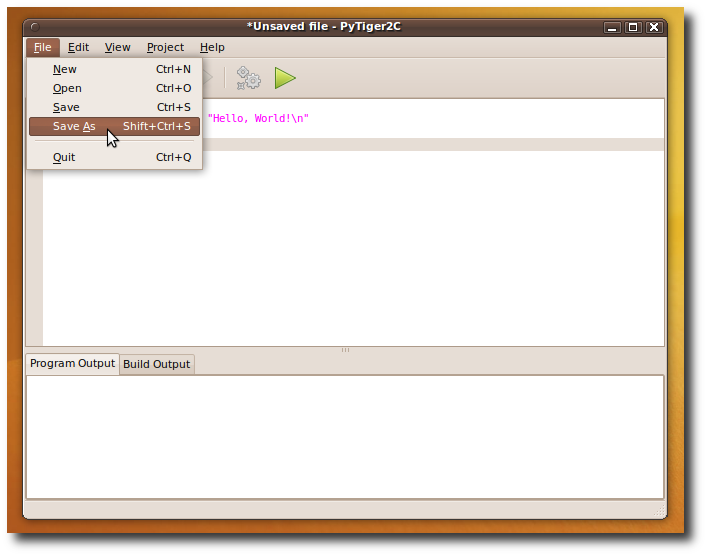
\includegraphics[width=5.5in]{gui/3-saving-as}
  \caption{Guardando el nuevo programa creado.}
  \label{fig:3-saving-as}
\end{figure}

\newpage

La acción anterior mostrará un diálogo donde se debe especificar el nombre que
deberá tener el archivo, el directorio donde se guardará  y confirmar utilizando
el botón \emph{Save As} como se ilustra en la figura~\ref{fig:4-save-as}.

\begin{figure}[htb]
  \centering
  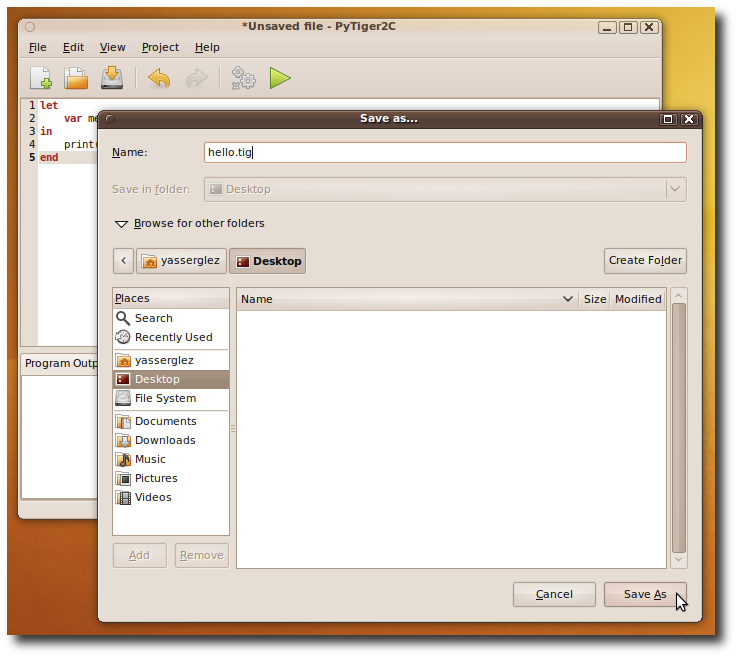
\includegraphics[width=6in]{gui/4-save-as}
  \caption{Introduciendo el nombre del nuevo archivo.}
  \label{fig:4-save-as}
\end{figure}

\newpage

Una vez guardado el nuevo programa Tiger en un archivo es posible compilarlo
utilizando el elemento \emph{Build} del menú \emph{Project} como se ilustra
en la figura~\ref{fig:5-building}.

\begin{figure}[htb]
  \centering
  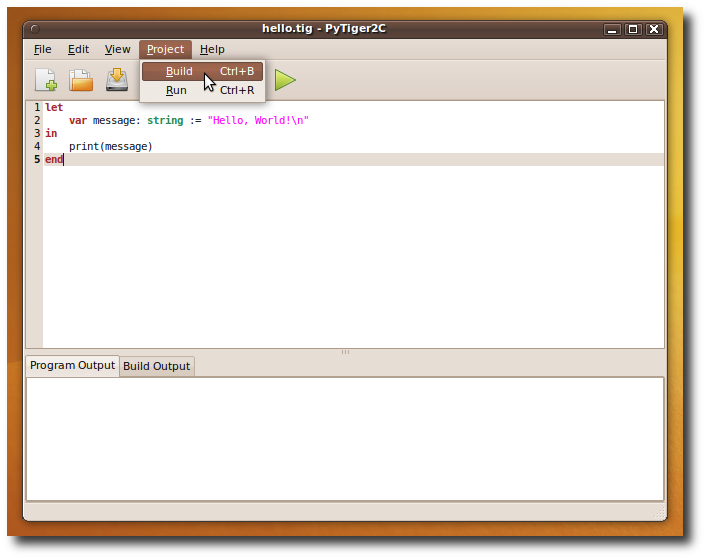
\includegraphics[width=5.5in]{gui/5-building}
  \caption{Compilando el nuevo programa.}
  \label{fig:5-building}
\end{figure}

\newpage

Si el programa Tiger no tiene ningún error se mostrará, en la pestaña
\emph{Build Output}, un mensaje indicando que el proceso de compilación
finalizó correctamente como se ilustra en la figura~\ref{fig:6-build-succeded}.

\begin{figure}[htb]
  \centering
  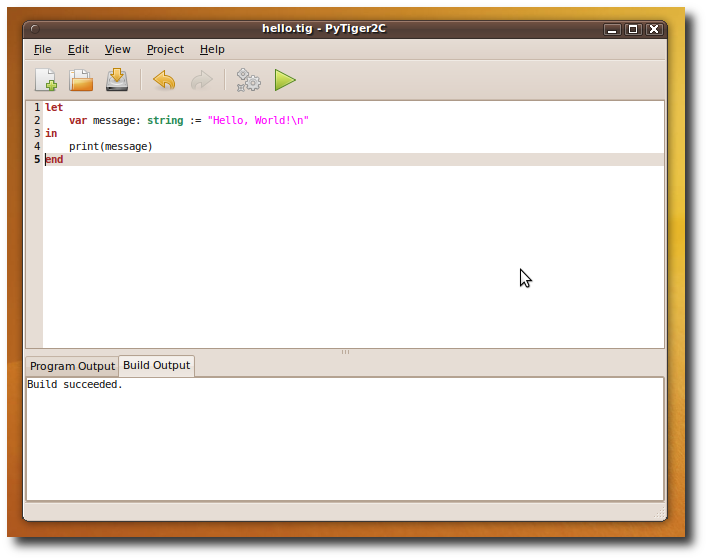
\includegraphics[width=5.5in]{gui/6-build-succeded}
  \caption{Mensaje indicando que el proceso de compilación finalizó
    correctamente.}
  \label{fig:6-build-succeded}
\end{figure}

\newpage

Si el programa Tiger tuviera algún error semántico o sintáctico se mostrarán
los mensajes correspondiente en la pestaña \emph{Build Output}. Por ejemplo,
la figura~\ref{fig:7-build-errors} muestra el mismo programa
\emph{Hello, World!} pero se ha sustituído el llamado a \texttt{print} de la
línea 4 por un llamado a \texttt{printi}; esto genera un error semántico
ya que la función \texttt{printi} recibe un \texttt{int} como argumento
y se está llamando con un argumento \texttt{string}.

\begin{figure}[htb]
  \centering
  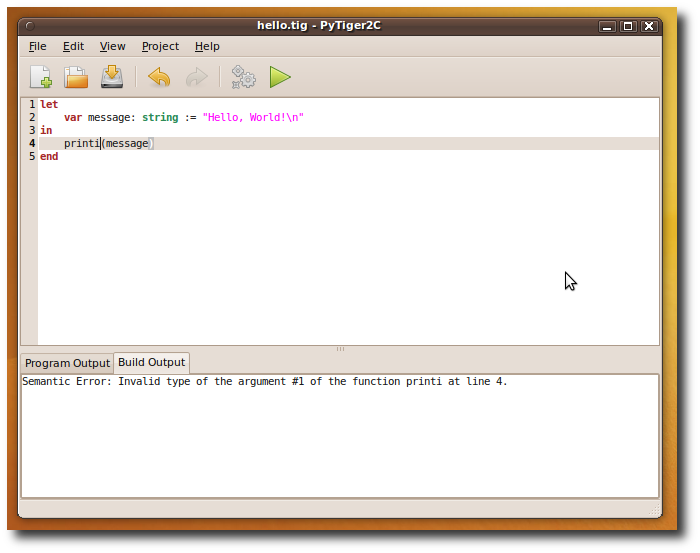
\includegraphics[width=5.5in]{gui/7-build-errors}
  \caption{Mensaje indicando los errores presentes en el programa.}
  \label{fig:7-build-errors}
\end{figure}

\newpage

Una vez que el programa se ha compilado correctamente es posible ejecutarlo
desde la interfaz gráfica utilizando el elemento \emph{Run} del menú
\emph{Project} como se ilustra en la figura~\ref{fig:8-running}.

\begin{figure}[htb]
  \centering
  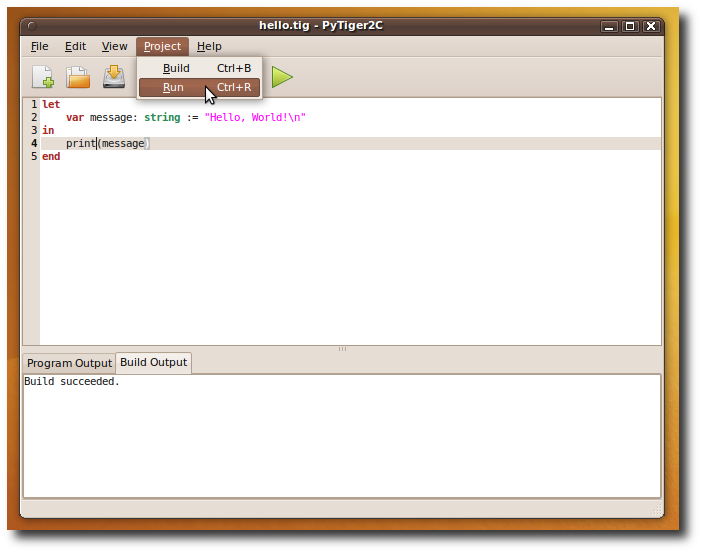
\includegraphics[width=5.5in]{gui/8-running}
  \caption{Ejecutando el nuevo programa.}
  \label{fig:8-running}
\end{figure}

\newpage

La salida \emph{standard} y de errores del programa se mostrará en la
pestaña \emph{Program Output} como se ilustra en la
figura~\ref{fig:9-program-output}.

\begin{figure}[htb]
  \centering
  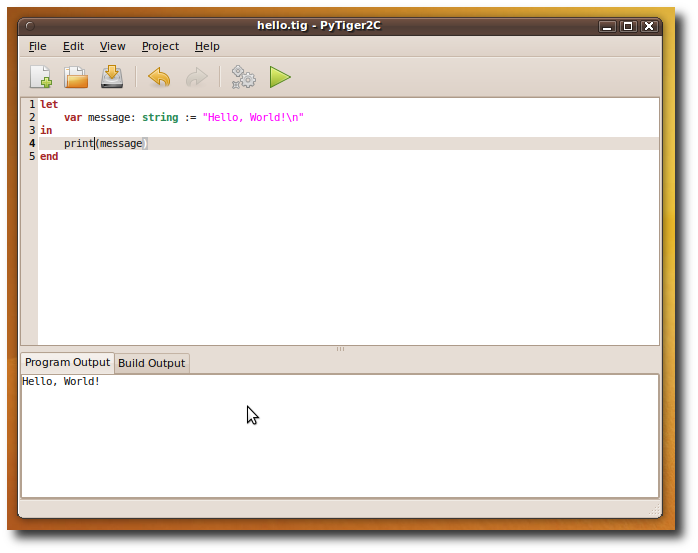
\includegraphics[width=5.5in]{gui/9-program-output}
  \caption{Salida del programa.}
  \label{fig:9-program-output}
\end{figure}

\newpage

Es posible ver el código C generado para el programa Tiger durante el proceso de
compilación. Para esto se utiliza el elemento \emph{C Code} del menú \emph{View}
como se ilustra en la figura~\ref{fig:10-viewing-code}. Al hacer esto, se mostrará
una ventana auxiliar con el código C como ilustra en la
figura~\ref{fig:11-code-viewer}.

\begin{figure}[htb]
  \centering
  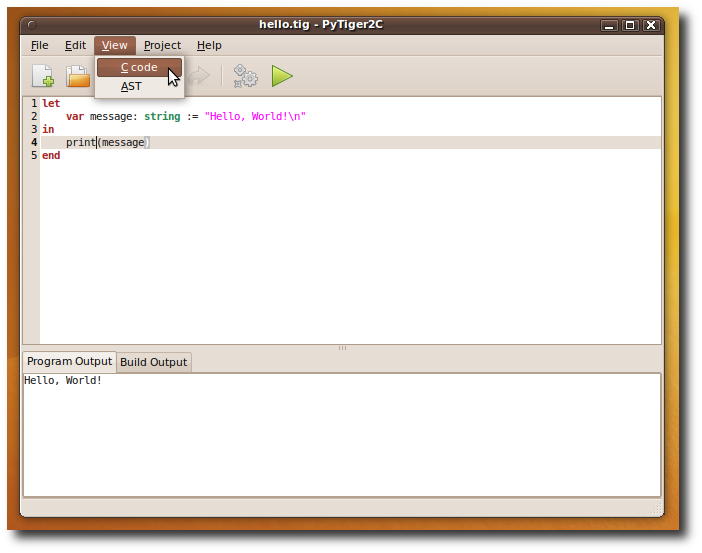
\includegraphics[width=5.5in]{gui/10-viewing-code}
  \caption{Ver el código C generado para el programa.}
  \label{fig:10-viewing-code}
\end{figure}

\begin{figure}[htb]
  \centering
  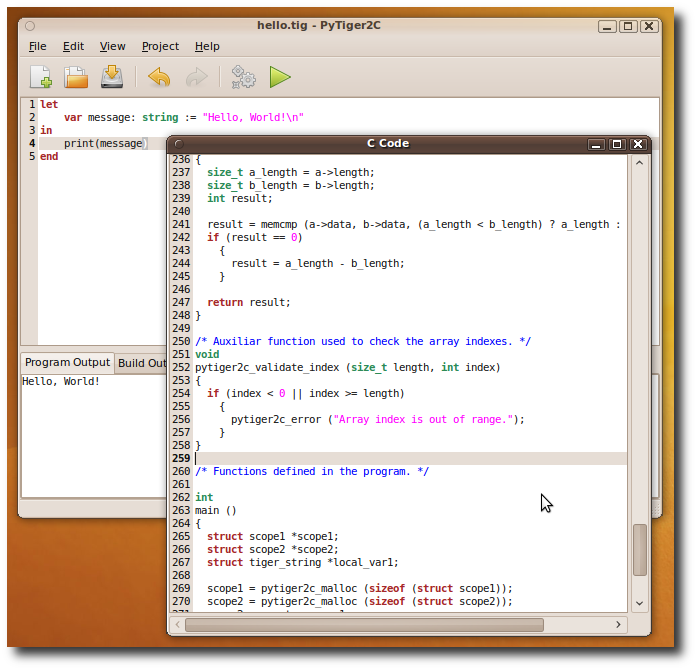
\includegraphics[width=5.5in]{gui/11-code-viewer}
  \caption{Ventana auxiliar mostrando el código C generado para el programa.}
  \label{fig:11-code-viewer}
\end{figure}

\newpage

La interfaz gráfica permite además ver el árbol de sintáxis abstracta
correspondiente al programa en edición. Esto puede hacerce mediante el
elemento \emph{AST} del menú \emph{View} como se ilustra en la
figura~\ref{fig:12-viewing-ast}. Al hacer esto, se mostrará una ventana
auxiliar con el árbol de sintáxis abstracta como se ilustra en la
figura~\ref{fig:13-ast-viewer}.

\begin{figure}[htb]
  \centering
  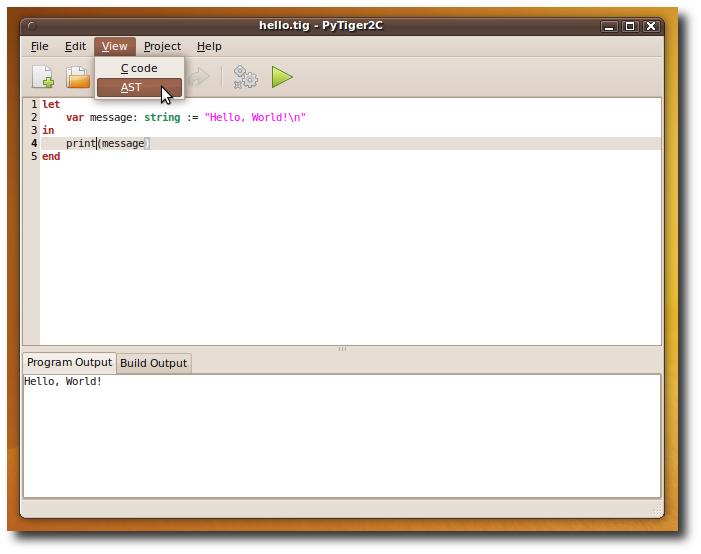
\includegraphics[width=5.5in]{gui/12-viewing-ast}
  \caption{Ver el árbol de sintáxis abstracta correspondiente al programa.}
  \label{fig:12-viewing-ast}
\end{figure}

\begin{figure}[htb]
  \centering
  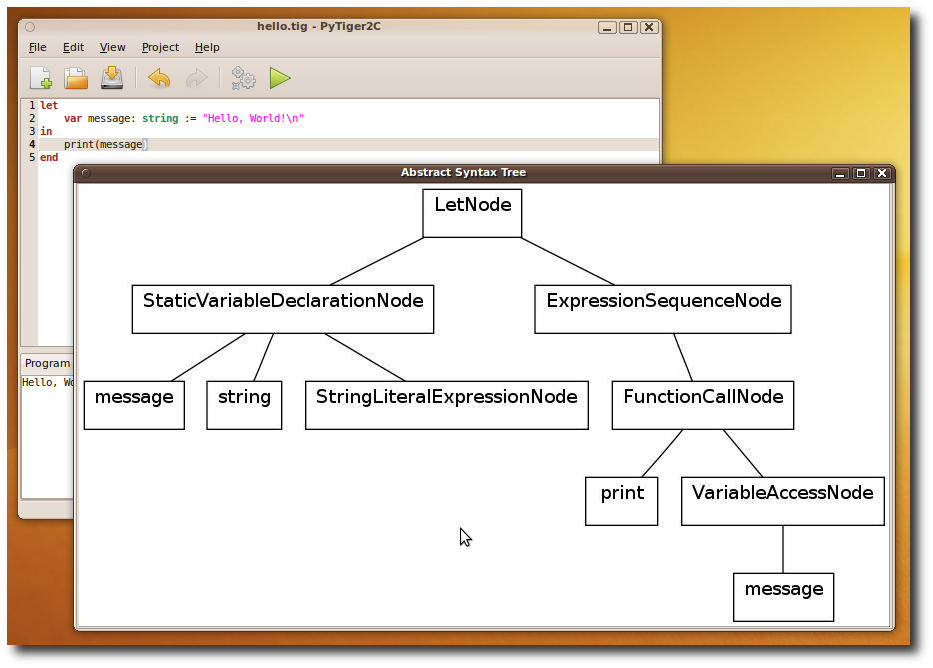
\includegraphics[width=6.5in]{gui/13-ast-viewer}
  \caption{Ventana auxiliar mostrando el árbol de sintáxis abstracta
    correspondiente al programa.}
  \label{fig:13-ast-viewer}
\end{figure}

\end{document}
